% geometry_and_trigonometry:x09 GDC:YES
\begin{question}
  \hspace*{\fill} [Note Maximale: 15]\par
  \noindent La figure ci-dessous représente un cercle de centre $O$ et de rayon $8\,cm$.\par
  \medskip
  \begin{center} % or flushleft or flushright
    \noindent La figure n'est pas à ĺ'échelle.\par
    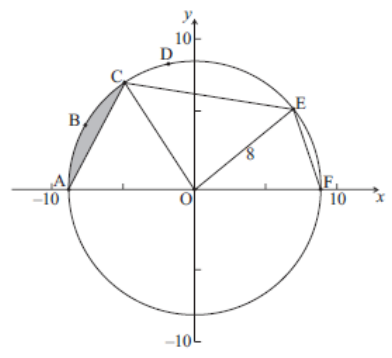
\includegraphics[scale=0.4]{figure_x9}\par
  \end{center} % or flushleft or flushright

  \noindent Les points $A$, $B$, $C$, $D$, $E$, $F$ sont sur le cercle, et $AF$ est un diamètre.  La longueur de l'arc $ABC$ es $6 cm$.\par
  \begin{enumerate}[label=(\alph*)]
    \item Trouvez la mesure de langle $\angle\,AOC$.\hspace*{\fill} [2]
    \item À partir de là, trouvez laire de la region grisée.\hspace*{\fill} [6]
    \item L'aire du secture $OCDE$ est de $45 cm^2$. Trouvez la mesure de langle $\angle COE$.\hspace*{\fill} [2]
    \item Trouvez $EF$.\hspace*{\fill} [5]
  \end{enumerate}
\end{question}
